\chapter{FFDA}

\section{Traccia}
Conduct the analysis for MercuryErrorLog.txt and BGLError-Log.txt:
\begin{itemize}
    \item tuple count plot + selected CWIN;
    \item grouping entries with selected CWIN;
    \item empirical reliabilities distributions;
    \item fit the empirical reliabilility (try all the models- exponential, hy-
perexponential, weibull);
\end{itemize}

Answer the following :
\begin{itemize}
    \item Can the same coalesce windows be used across different
nodes (Mercury, BG/L) and error categories (Mercury) ?
    \item  What about the relationship between the system reliability
and nodes reliability?
    \item there exist dependability-bottlenecks (i.e., topcontributors to the total number of failures)?
    \item Do similar functional nodes (e.g., two Mercury tg-cX computing nodes or BG/L I/O nodes Ri:Mx:Nz) exhibit similar reliability parameters?
    \item there exist a relationship between the error types and the node (Mercury)?
\end{itemize}

\newpage
\section{Mercury}
Il super-calcolatore \textit{Mercury} consiste in una serie di nodi organizzati in un'architettura a tre livelli a cui si aggiunge un nodo di management (\cref{fig:mercury_arch}).

\begin{figure}[H]
    \centering
    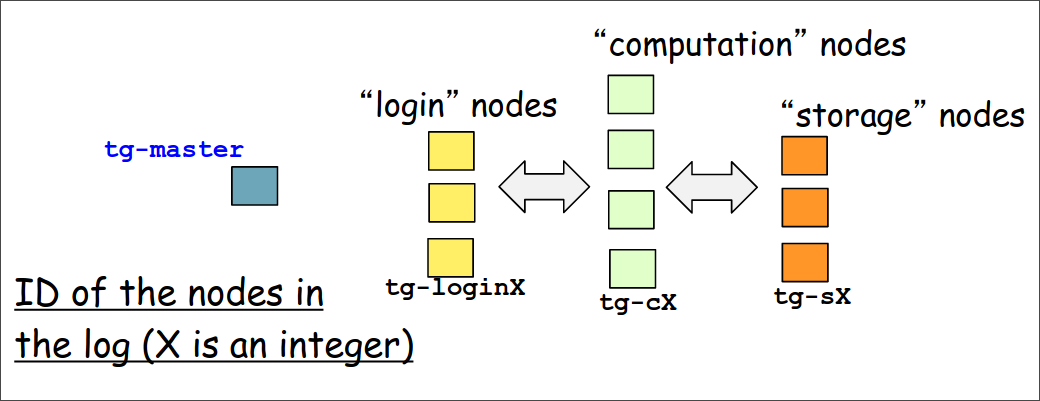
\includegraphics[width=0.8\textwidth]{img/ch6/mercury_architecture.png}
    \caption{Architettura multi-livello del supercal-calcolatore Mercury}
    \label{fig:mercury_arch}
\end{figure}

Gli altri nodi sono:
\begin{itemize}
    \item Login;
    \item Computation;
    \item Storage;
\end{itemize}

Il file in ingresso MercuryErrorLog.txt contiene $80854$ entry ciascuna delle quali ha il formato \textit{timestamp - nodo - categoria - messaggio di errore}.


\subsection{Temporal coalescence }
Partendo dal file dei log si vuole diminuire il numero di entries raggruppando quelle che possono essere relative allo stesso fault. Per farlo è stata applicata la tecnica della coalescenza temporale in cui, una definita una finestra temporale $W$, si pongono all'interno della stessa tupla tutti gli eventi con differenza di timestamp minore di $W$ come scritto nella \cref{eq:coal_window}.

\begin{equation}
    X(t+1) - X(t) < W
    \label{eq:coal_window}
\end{equation}

La difficoltà principale nell'utilizzo di questa tecnica è il calcolo della \textit{window size}.
Nel caso sia troppo piccola porta a dei fenomeni di \textit{trucation} (\cref{fig:ex_truncation}), in cui eventi relativi allo stesso fault vengono messi in tuple diverse, e viceversa si possono verificare \textit{collisions} ( (\cref{fig:ex_collision}) con $W$ troppo grandi, in cui eventi relativi a fault diversi vengono raggruppati insieme.

\begin{figure}[H]
    \centering
    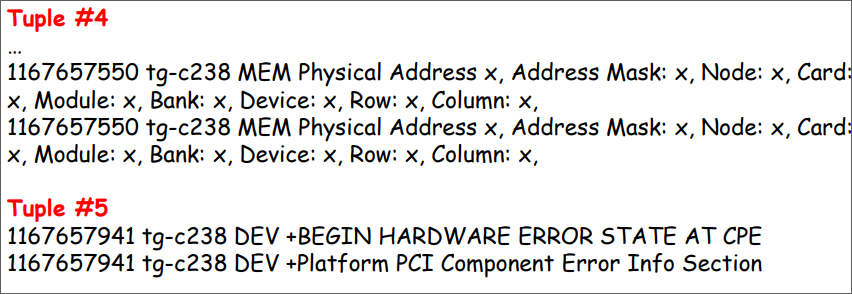
\includegraphics[width=0.8\textwidth]{img/ch6/ex_truncation.png}
    \caption{Esempio di truncation}
    \label{fig:ex_truncation}
\end{figure}

\begin{figure}[H]
    \centering
    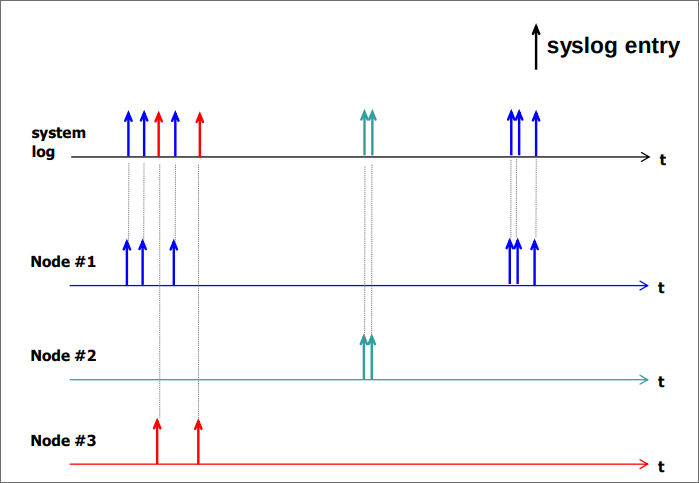
\includegraphics[width=0.8\textwidth]{img/ch6/ex_collision.png}
    \caption{Esempio di collisione}
    \label{fig:ex_collision}
\end{figure}

Per trovare un valore ottimale di W è stata effettuata una \textit{Sensitivity Analysis}, calcolando il numero di tuple generate a seconda di multipli valori della \textit{window size}.

Il risultato ottenuto è visibile in figura \cref{fig:mercury_cwin}.

\begin{figure}[H]
    \centering
    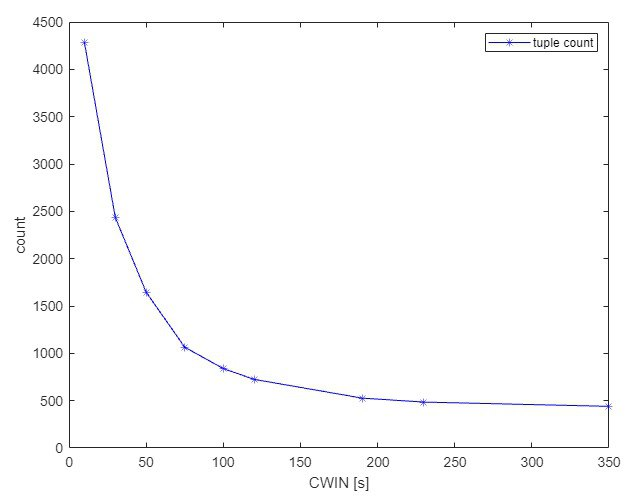
\includegraphics[width=0.8\textwidth]{img/ch6/merc_cwin.png}
    \caption{}
    \label{fig:mercury_cwin}
\end{figure}

Porsi leggermente a destra del punto di knee porta i risultati ottimali, e sono stati scelti due valori per $W$:
\begin{itemize}
    \item $W_1=180$
    \item $W_2=220$
\end{itemize}

Per entrambe le \textit{window size} sono state generate le tuple e le seguenti statistiche:
\begin{itemize}
    \item Interarrivals: tempi di interarrivo tra le tuple (TTF).
    \item Starting points: timestamp del punto di inizio della tupla.
    \item Lengths: durata dei fallimenti e quindi la lunghezza delle singole tuple.
\end{itemize}


\subsection{Reliability}

È possibile stimare la reliability del sistema in maniera empirica utilizzando il $TTF$ calcolato a partire dagli \textit{interarrivals} ottenuti nella sezione precedente. 
In \cref{fig:merc_reliability} è possibile notare come la reliability con $W=220$ sia migliore di quella con $W=180$. 
\begin{figure}[H]
    \centering
    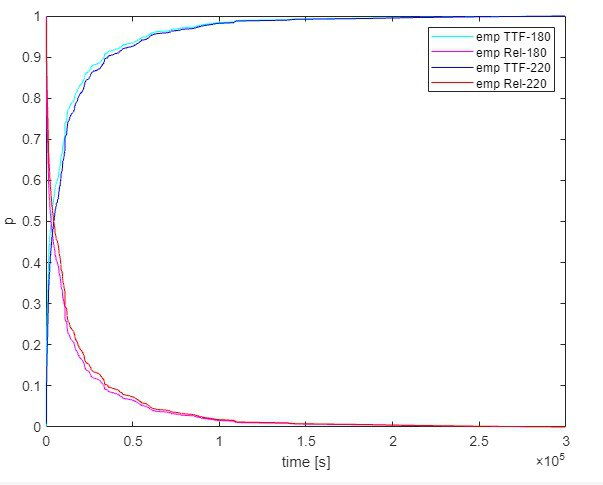
\includegraphics[width=\textwidth]{img/ch6/merc_ttf.png}
    \caption{Reliability Mercury con $W=180$ e $W=220$}
    \label{fig:merc_reliability}
\end{figure}

In seguito, è stata effettuata un'analisi per trovare la distribuzione che meglio rappresenta la Reliability empirica, con lo scopo di comprendere la natura dei fallimenti presenti nel sistema.

In particolare, è stato provato il \textit{fitting} per le seguenti distribuzioni:
\begin{itemize}
    \item \textbf{Esponenziale} (\cref{fig:merc_fit_exp}): i fallimenti sono \textit{memory less} e con \textit{failure rate} costante;
    \item \textbf{Iper-esponenziale}(\cref{fig:merc_fit_iperexp}): i fallimenti sono dovuti a più cause tra loro indipendenti;
    \item \textbf{Weibull}(\cref{fig:merc_fit_weibull}): con questa
    distribuzione si modellano i fallimenti con memoria di componenti
    elettronici;
\end{itemize}

\begin{figure}[H]
    \centering
    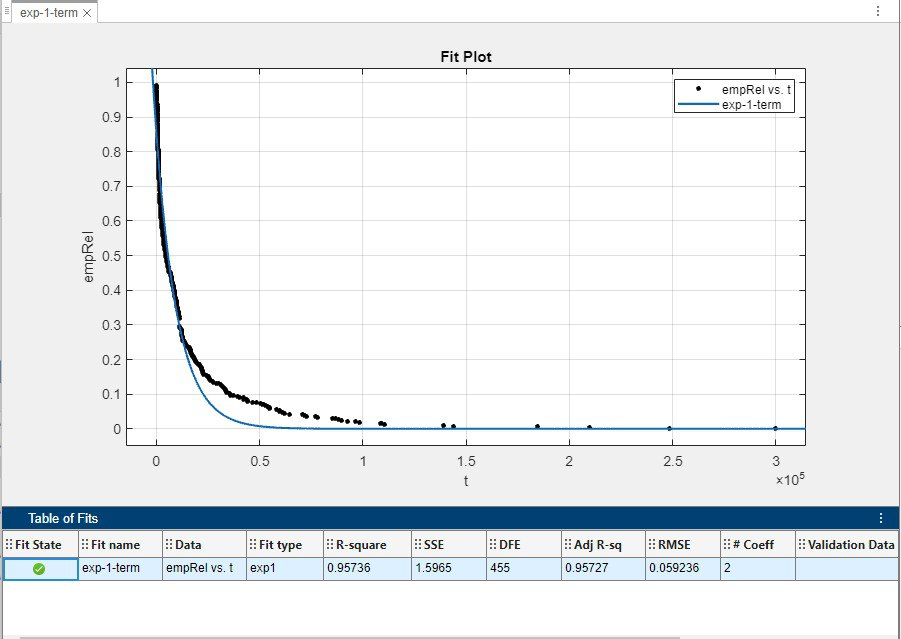
\includegraphics[width=\textwidth]{img/ch6/merc_fit_exp.png}
    \caption{Fit realiability Mercury con una distribuzione esponenziale}
    \label{fig:merc_fit_exp}
\end{figure}

\begin{figure}[H]
    \centering
    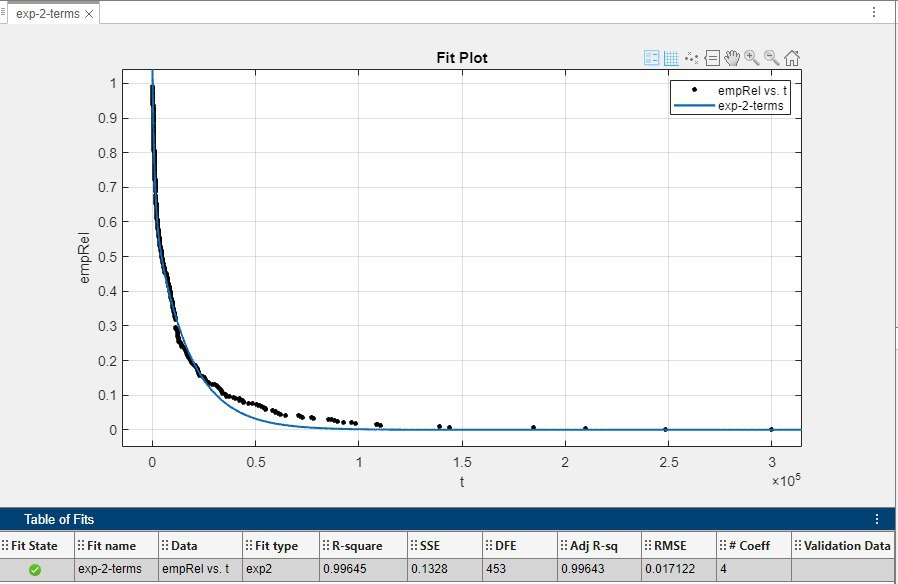
\includegraphics[width=\textwidth]{img/ch6/merc_fit_iperexp.png}
    \caption{Fit realiability Mercury con una distribuzione iper-esponenziale}
    \label{fig:merc_fit_iperexp}
\end{figure}

\begin{figure}[H]
    \centering
    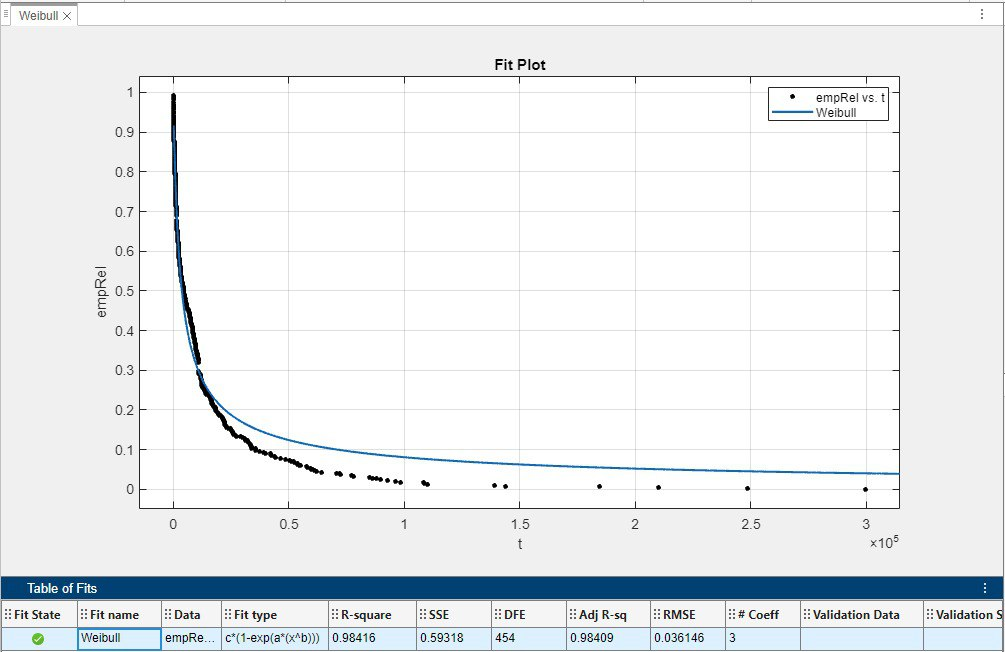
\includegraphics[width=\textwidth]{img/ch6/merc_fit_weibull.png}
    \caption{Fit realiability Mercury con una distribuzione weibull}
    \label{fig:merc_fit_weibull}
\end{figure}


\begin{table}[H]
\centering
    \begin{tabular}{|c|c|c|}
    \hline
    \multicolumn{1}{|c|}{\textbf{Curva}} &
    \multicolumn{1}{|c|}{\textbf{$R^2$}} &
    \multicolumn{1}{|c|}{\textbf{SSE}}
    \tabularnewline \hline

Esponenziale & $0.9573$ & $1.5965$   \tabularnewline \hline
Iper-esponenziale & $0.9964$ &  $0.1328$  \tabularnewline \hline
Weibull & $0.9841$ &  $0.5931$  \tabularnewline \hline
\end{tabular}
\caption{$R^2$ e SSE ottenuti dal fitting delle distribuzioni esponenziali, iper-esponenziali e Weibull}
\label{tab:merc_fit_parameters}
\end{table}

A valle della valutazione effettuata, osservando l'\textit{R-Square} e SSE in \cref{tab:merc_fit_parameters},  è possibile affermare che la distribuzione che meglio approssima la reliability empirica è una iper-esponenziale. 

Come ulteriore conferma è stato effettuato il test di Kolmogorov-Smirnov per le tre distribuzioni.

\begin{table}[H]
\centering
    \begin{tabular}{|c|c|c|}
    \hline
    \multicolumn{1}{|c|}{\textbf{Curva}} &
    \multicolumn{1}{|c|}{\textbf{H}} &
    \multicolumn{1}{|c|}{\textbf{P-Value}}
    \tabularnewline \hline

Esponenziale & $1$ & $0.68 \cdot10^{-4}$   \tabularnewline \hline
Iper-esponenziale & $0$ &  $0.7105$  \tabularnewline \hline
Weibull & $0$ &  $0.153$  \tabularnewline \hline
\end{tabular}
\caption{Esito test Kolmogorov-Smirnov}
\label{tab:ks_mercury}
\end{table}


\subsection{Analisi Collisions \& Truncations}

Proseguendo con $W=220$, sono state effettuate analisi per trovare collisioni e troncamenti all'interno delle tuple.

Per trovare una probabile collisione sono state esaminate le tuple a lunghezza maggiore, cercando eventi apparentemente slegati tra loro. 

Una probabile collisione è mostrata in \cref{fig:merc_collision} nella tupla 322, dove è possibile notare eventi relativi ai nodi di computazione \textit{tg-c401} e \textit{tg-c669} insieme a quelli del nodo di login \textit{tg-login3}, apparentemente slegati tra loro.
\begin{figure}[H]
    \centering
    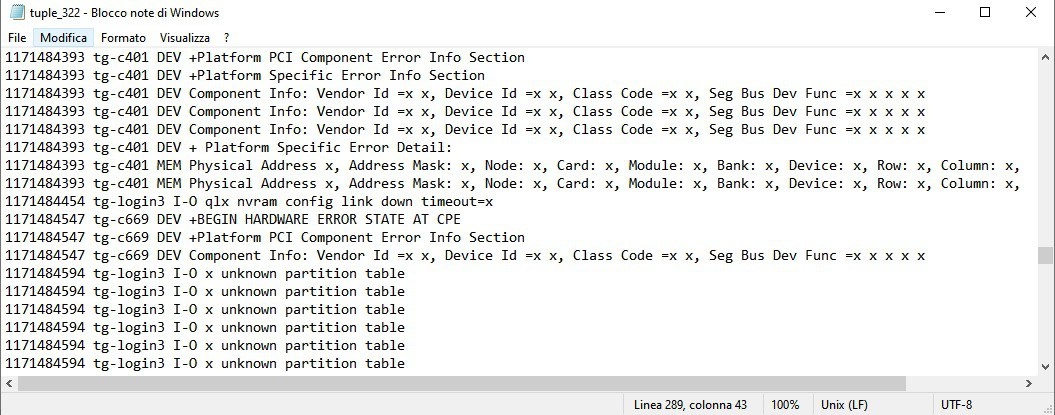
\includegraphics[width=\textwidth]{img/ch6/merc_collision.png}
    \caption{Esempio di probabile collisione per Mercury con $W=220$}
    \label{fig:merc_collision}
\end{figure}


Un esempio di probabile \textit{truncation} è mostrato in \cref{fig:merc_truncation}, dove è possibile notare che nelle tuple $66,67,68$ è presente lo stesso tipo di errore, di tipo NET, relativo allo stesso nodo \textit{tg-master}. 
\begin{figure}[H]
    \centering
    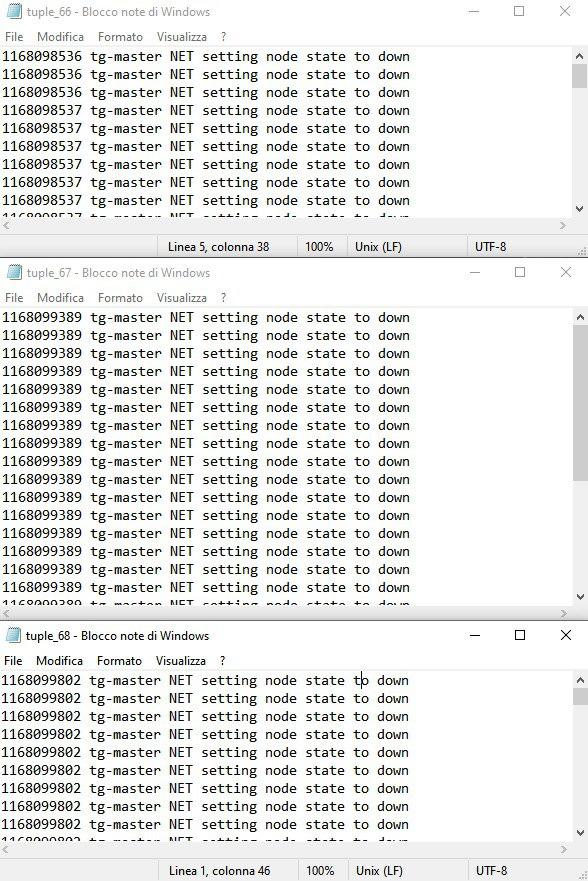
\includegraphics[width=0.8\textwidth]{img/ch6/merc_truncation.png}
    \caption{Esempio di probabile troncamento per Mercury con $W=220$}
    \label{fig:merc_truncation}
\end{figure}


\subsection{Ulteriori Analisi}

 \paragraph{Studio della Window size per nodi e categorie}
 Si vuole stabilire se sia possibile usare la stessa $W$ per i diversi nodi e le categorie di Mercury. 

Dopo una fase di filtraggio sono stati identificati i quattro nodi con più errori del sistema, ed è stata svolta una sensitivity analysis simile a quella presente nelle sezioni precedenti. 
I nodi scelti sono:
\begin{itemize}
    \item tg-c401
    \item tg-c572
    \item tg-master
    \item tg-s044
\end{itemize}


Dai risultati in \cref{fig:comp_windows-size_per-nodo} è possibile notare come per i diversi nodi non sia possibile scegliere una \textit{window size} unica e ottimale. 

\begin{figure}[H]
    \centering
    \begin{subfigure}{.5\textwidth}
        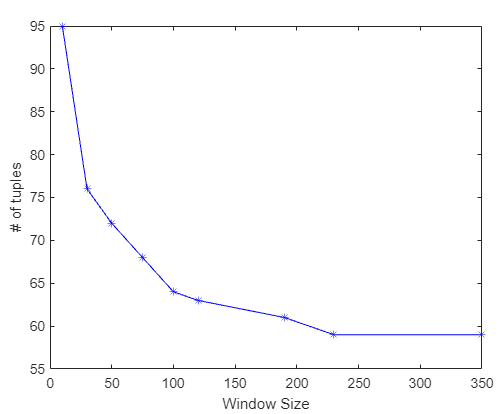
\includegraphics[width=\linewidth]{img/ch6/merc_cmaster-wsize.png}
        \caption{Nodo tg-master}
    \end{subfigure}\hfil
    \begin{subfigure}{.5\textwidth}
         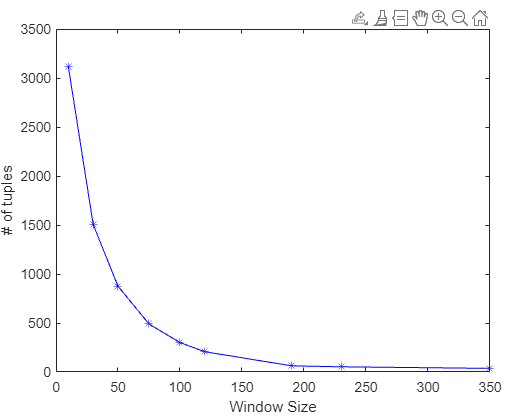
\includegraphics[width=\textwidth]{img/ch6/merc_c401-wsize.png}
         \caption{Nodo tg-c401}
    \end{subfigure}

    \begin{subfigure}{.5\textwidth}
        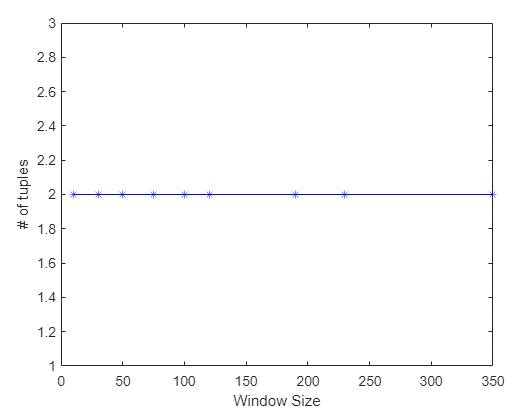
\includegraphics[width=\linewidth]{img/ch6/merc_c572-wsize.png}
        \caption{Nodo tg-master}
    \end{subfigure}\hfil
    \begin{subfigure}{.5\textwidth}
         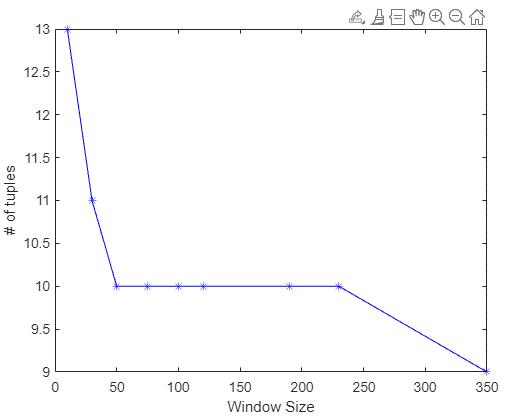
\includegraphics[width=\textwidth]{img/ch6/merc_s044-wsize.png}
         \caption{Nodo tg-c401}
    \end{subfigure}

    \caption{Comparazione window size per nodo}
    \label{fig:comp_windows-size_per-nodo}
\end{figure}


Per quanto riguarda invece le categorie di errore i risultati sono mostrati in \cref{eq:coal_window}, analizzando sempre le prime quattro in termini di numero di errori:
\begin{itemize}
    \item DEV
    \item IO
    \item NET
    \item MEM
    \item PRO
\end{itemize}

In questo caso una finestra vicina a 220 potrebbe andare bene per le categorie DEV, MEM e NET, ma risulta inadatta per I/O e PRO. 

\begin{figure}[H]
    \centering
    \begin{subfigure}{.5\textwidth}
        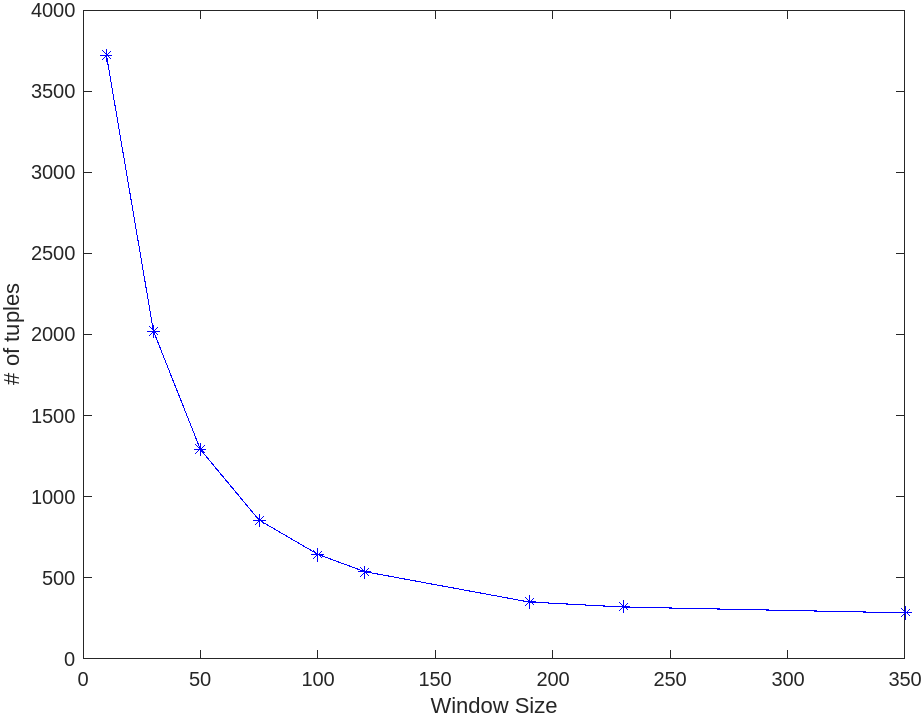
\includegraphics[width=\linewidth]{img/ch6/merc_dev-wsize.png}
        \caption{Categoria DEV}
    \end{subfigure}\hfil
    \begin{subfigure}{.5\textwidth}
         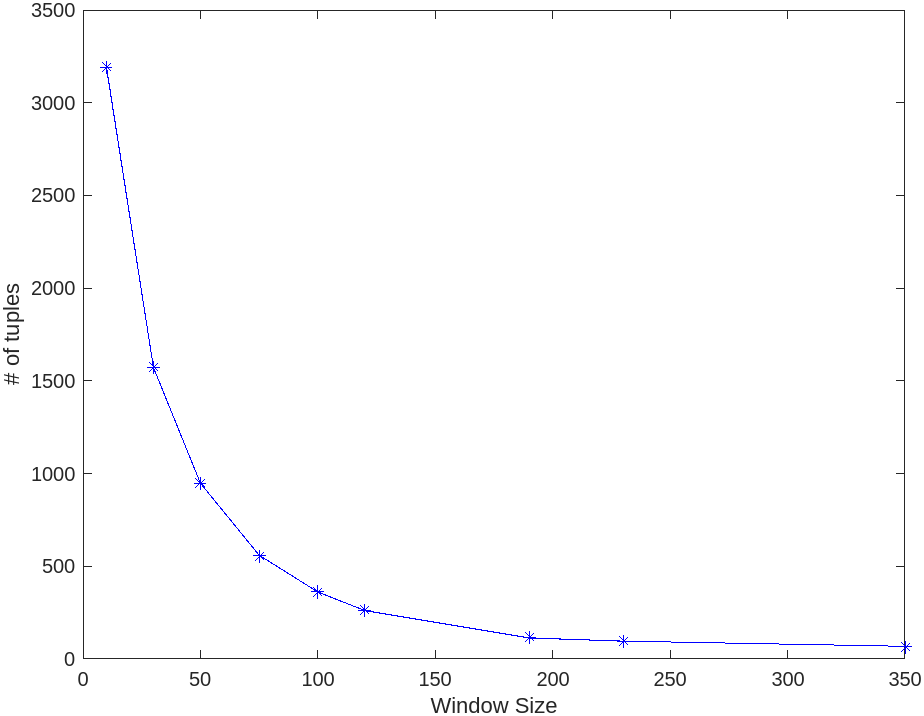
\includegraphics[width=\textwidth]{img/ch6/merc_mem-wsize.png}
         \caption{Catergoria MEM}
    \end{subfigure}

    \begin{subfigure}{.5\textwidth}
        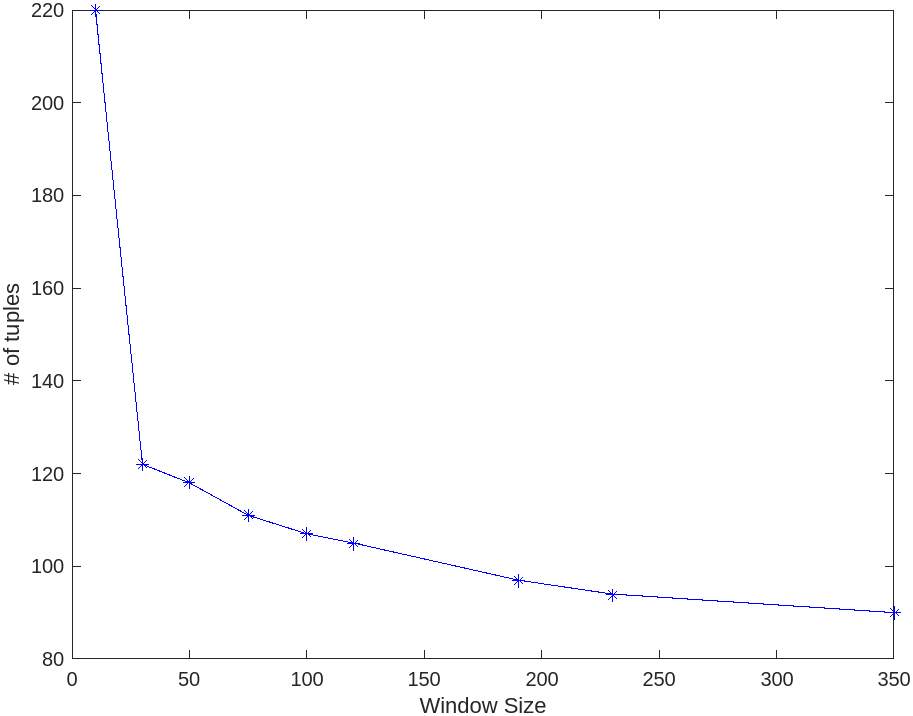
\includegraphics[width=\linewidth]{img/ch6/merc_io-wsize.png}
        \caption{Catergoria I/O}
    \end{subfigure}\hfil
    \begin{subfigure}{.5\textwidth}
         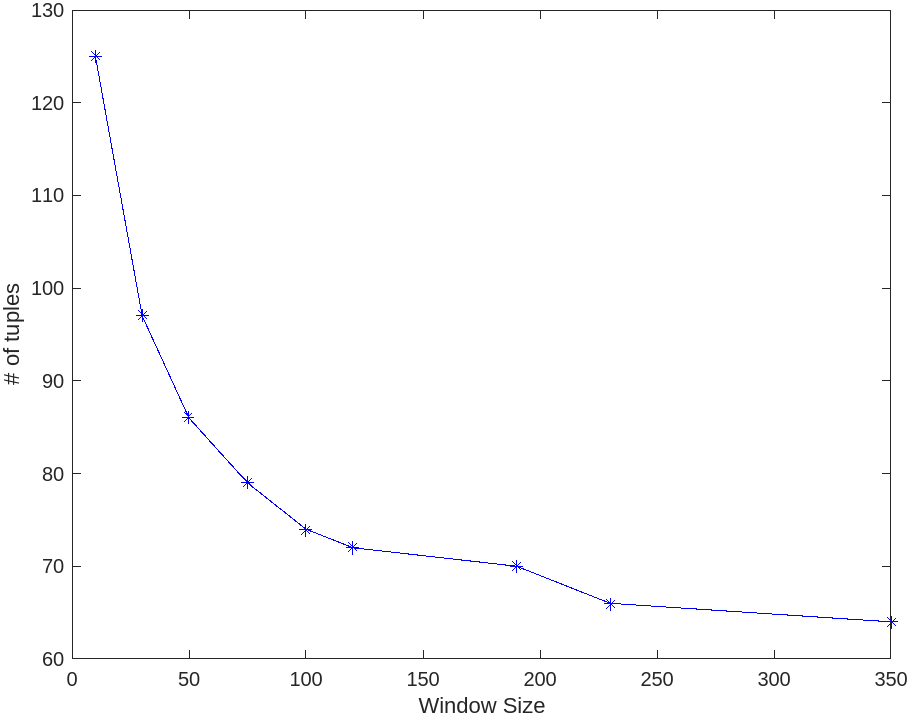
\includegraphics[width=\textwidth]{img/ch6/merc_net-wsize.png}
         \caption{Catergoria NET}
    \end{subfigure}

    \begin{subfigure}{.6\textwidth}
         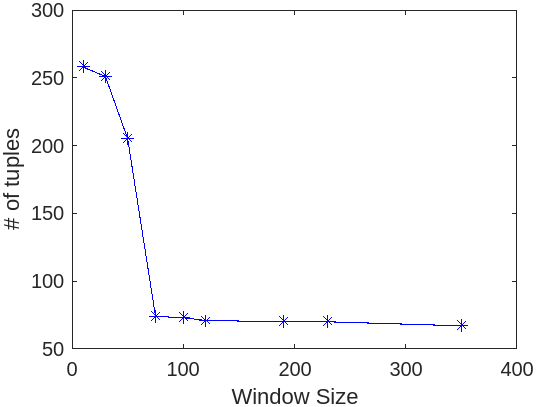
\includegraphics[width=\textwidth]{img/ch6/merc_pro-wsize.png}
         \caption{Catergoria PRO}
    \end{subfigure}

    \caption{Comparazione window size per categorie}
\end{figure}


\paragraph{Relazione tra system reliability e node reliability}

Al fine di comparare la reliability del sistema a quella dei nodi è stata effettuata un'analisi del TTF-empirico per questi ultimi, a partire dagli interarrivals filtrati. 

Come nelle sezioni precedenti, è stata effettuata in seguito una procedura di fitting, al termine della quale sono state individuate $4$ curve iper-esponenziali, rappresentanti le reliability dei nodi.

In \cref{fig:merc_rel_comp} è possibile notare come il nodo computazionale C401 abbia una reliability peggiore di quella del sistema totale, tant'è vero che la maggior parte degli errori nei log sono suoi.
Gli altri nodi si trovano al di sopra della reliability del sistema a partire da un certo istante di tempo.
Si noti che il nodo C572 non è presente nel grafico poichè, essendo composto da sole due tuple, non è stato possibile effettuare il fitting o rappresentarlo graficamente. 

\begin{figure}[H]
    \centering
    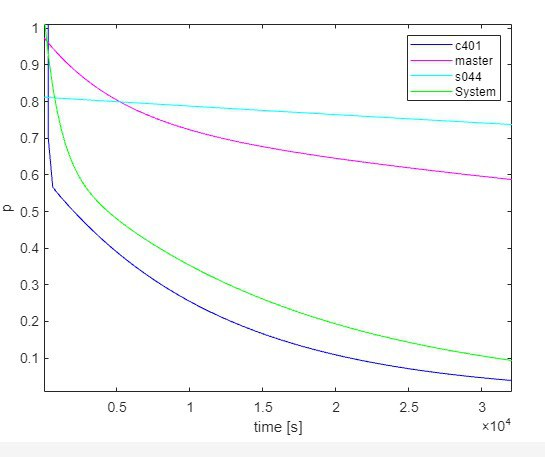
\includegraphics[width=\textwidth]{img/ch6/merc_rel_comp.png}
    \caption{Comparazione reliability del sistema Mercury con quella dei $4$ nodi analizzati}
    \label{fig:merc_rel_comp}
\end{figure}


\paragraph{Dependability Bottleneck}

Come mostrato nelle sezioni precedenti, il nodo che più contribuisce al numero di errori, e che peggiora la reliability del sistema generale è C401.

In \cref{fig:merc_error} si può notare che il nodo C401 contribuisce per più del 77\% degli errori.

\begin{figure}[H]
    \centering
    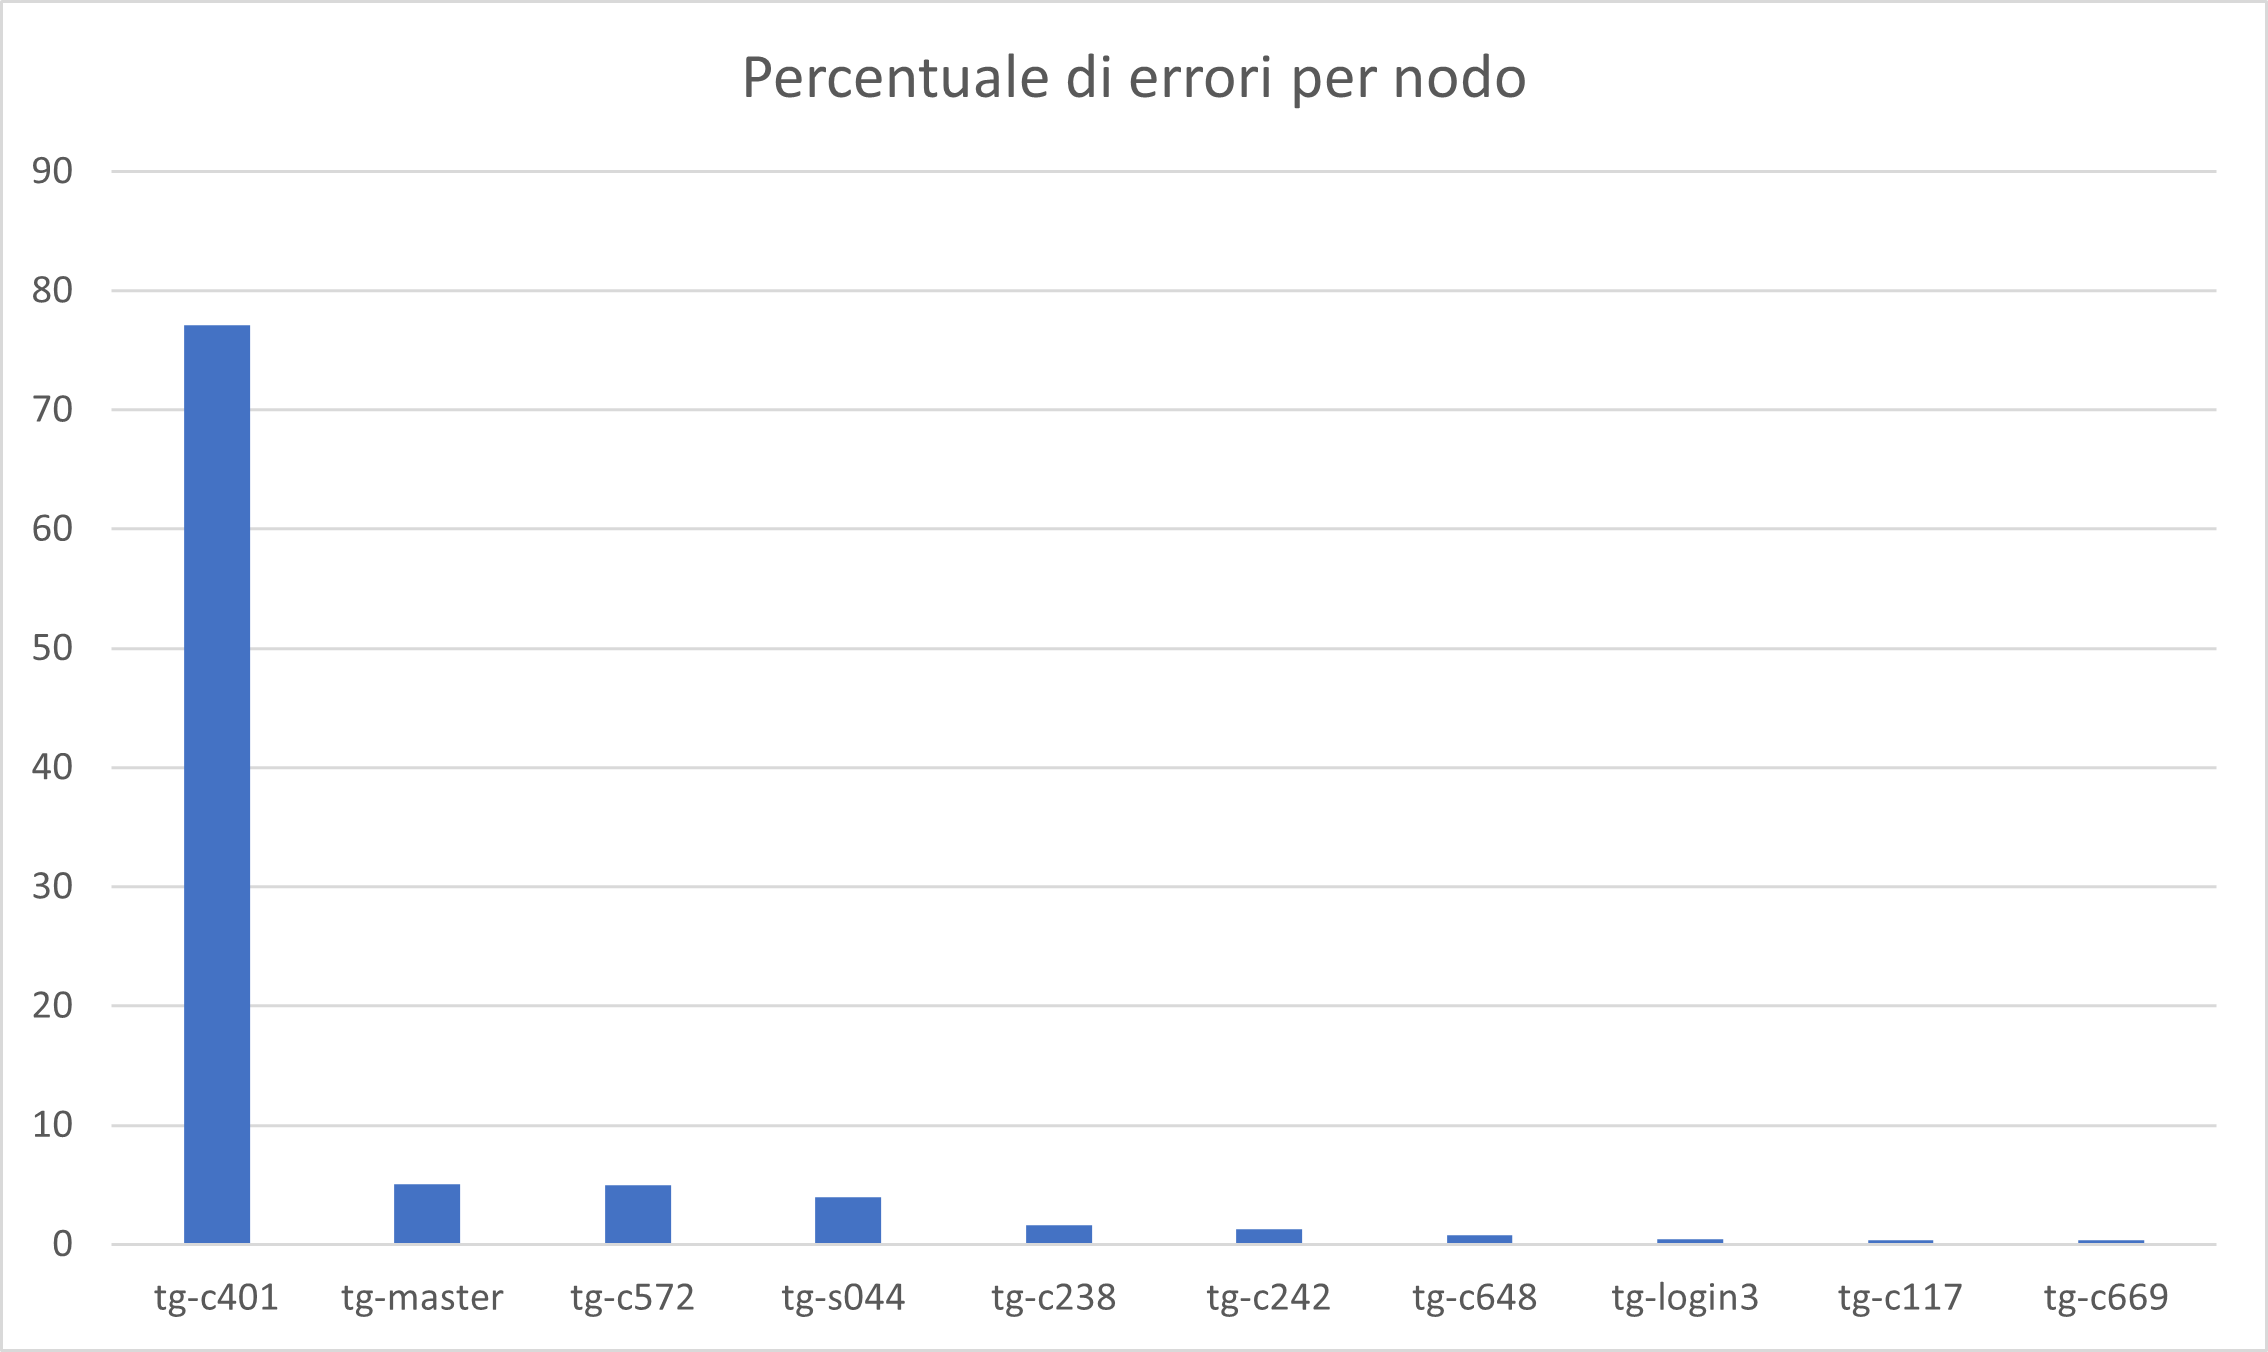
\includegraphics[width=\textwidth]{img/ch6/merc_errori.png}
    \caption{Percentuale di errori per nodo}
    \label{fig:merc_error}
\end{figure}

\paragraph{Reliability di nodi dello stesso tipo}

Sono stati esaminati due nodi di tipo computazionale:
\begin{itemize}
    \item C401
    \item C238
\end{itemize}

Dopo aver trovato la reliability empirica, ed aver fatto il fitting su una distribuzione iper-esponenziale, è possibile notare che, nonostante le differenze nell'andamento della curva vicino l'origine, la gran parte dei punti esaminati si trova sul tratto verticale che fa scendere quasi immediatamente la reliability. In questo senso si possono dire comparabili, anche se ovviamente C401 contribuisce per un numero molto maggiori di errori. 


\begin{figure}[H]
    \centering
    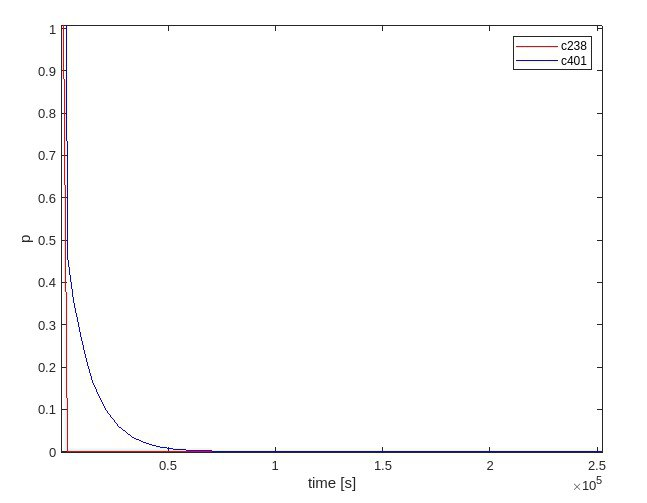
\includegraphics[width=0.8\textwidth]{img/ch6/merc_comp_c238vs401.png}
    \caption{Confronto reliability nodo \textit{tg-c401} e nodo \textit{tg-c238}}
    \label{fig:c238vsc401}
\end{figure}

\paragraph{Relazione tra tipo di errore e nodo}

Analizzando i \textit{fault} per categoria si trova che i nodi computazionali sono responsabili per la maggior parte degli errori di tipo \textit{DEV}, \textit{MEM} e \textit{PRO} (\cref{fig:err_calc_node}). Gli errori relativi alla rete (NET) sono per la maggior parte generati dal nodo \textit{tg-master} (\cref{fig:err_calc_node}).

Per quanto riguarda gli errori di tipo I/O, si può notare che sono dovuti principalmente al nodo di storage \textit{tg-s044} (\cref{fig:err_storage_node}), con la parte rimanente bilanciata tra altri tipi di nodi.

\begin{figure}[H]
    \centering
    \begin{subfigure}{.5\textwidth}
        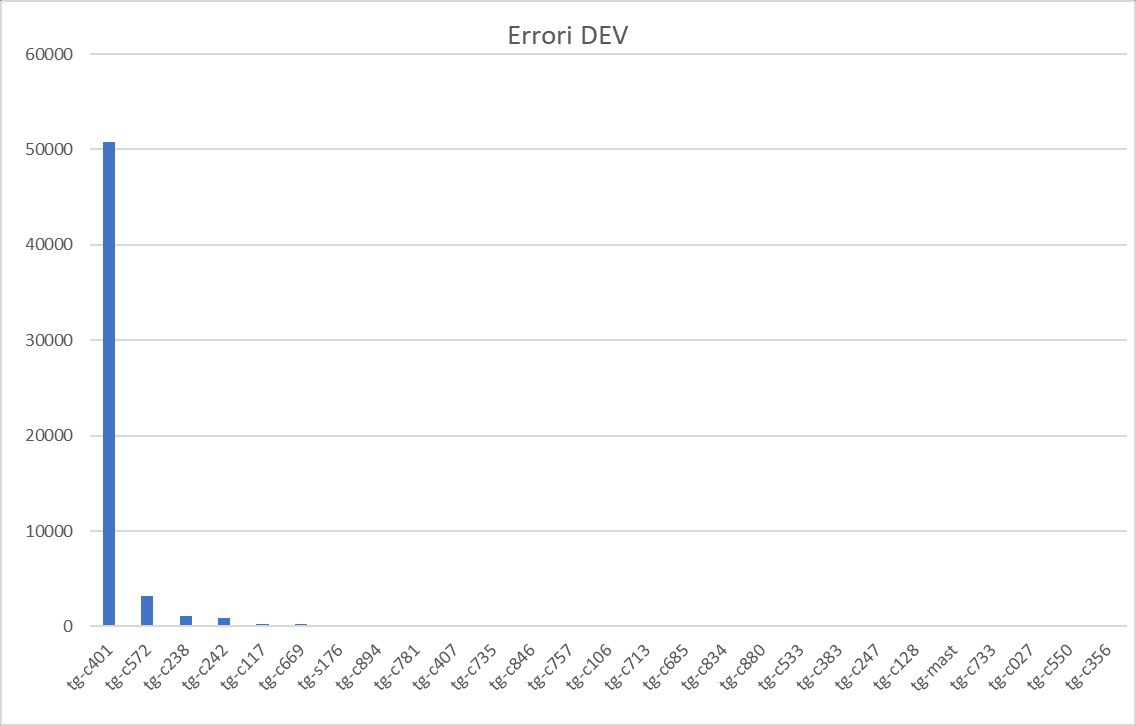
\includegraphics[width=\linewidth]{img/ch6/merc_dev_by_node.png}
        \caption{Errori tipo DEV}
    \end{subfigure}\hfil
    \begin{subfigure}{.5\textwidth}
        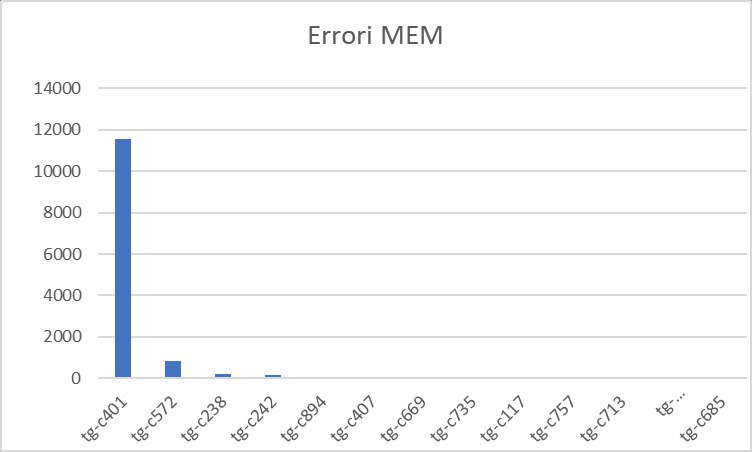
\includegraphics[width=\linewidth]{img/ch6/merc_mem_by_node.png}
        \caption{Errori tipo MEM}
    \end{subfigure}
    \begin{subfigure}{.6\textwidth}
        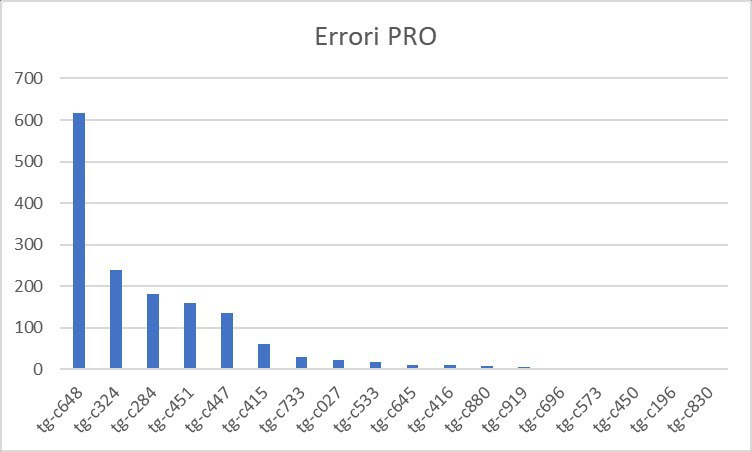
\includegraphics[width=\linewidth]{img/ch6/merc_pro_by_node.png}
        \caption{Errori tipo PRO}
    \end{subfigure}
    \caption{Errori di cui sono maggiormente responsabili i nodi di calcolo}
    \label{fig:err_calc_node}
\end{figure}


\begin{figure}[H]
    \centering
    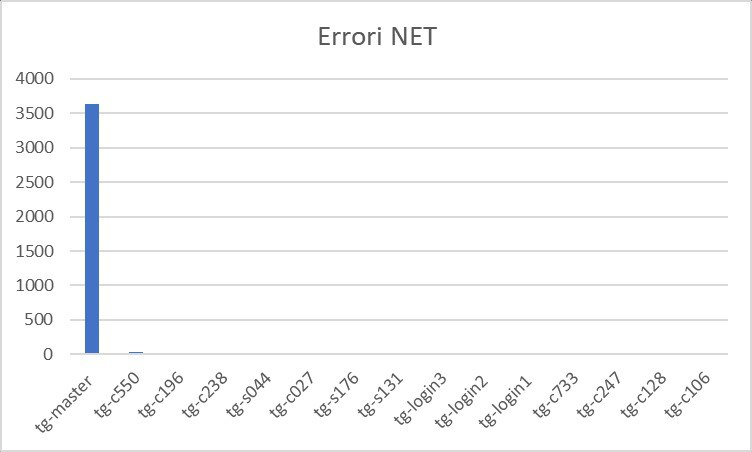
\includegraphics[width=0.9\textwidth]{img/ch6/merc_net_by_node.png}
    \caption{Errori di tipo NET}
    \label{fig:err_master_node}
\end{figure}


\begin{figure}[H]
    \centering
    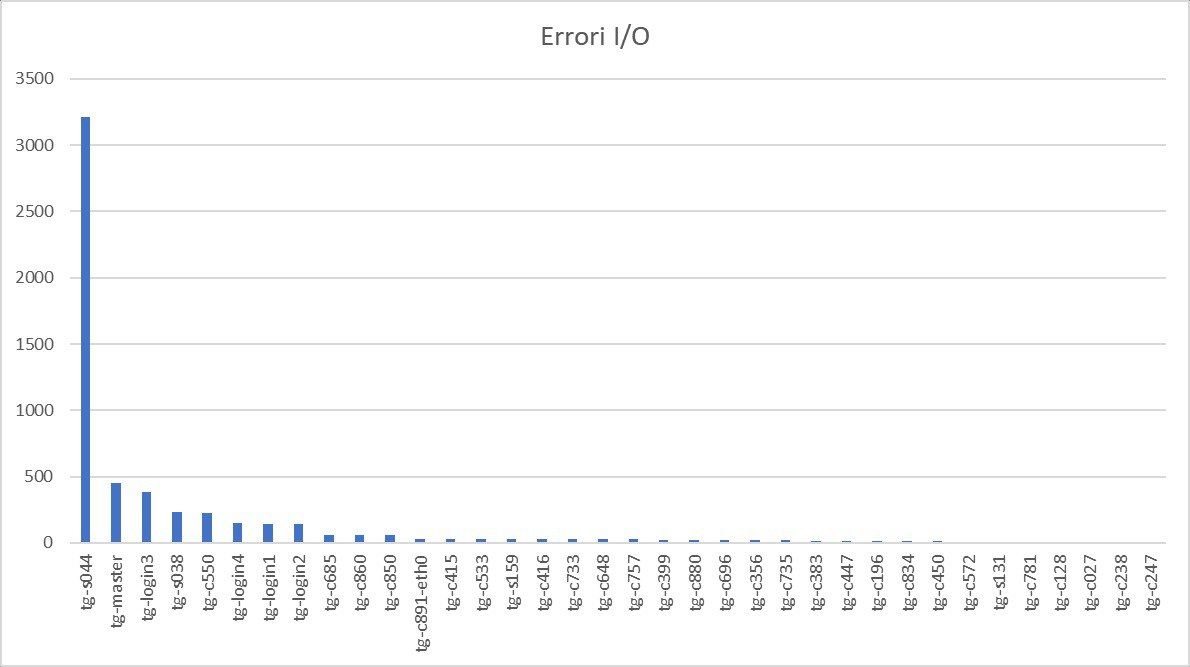
\includegraphics[width=0.9\textwidth]{img/ch6/merc_io_by_node.png}
    \caption{Errori di tipo I/O}
    \label{fig:err_storage_node}
\end{figure}

\clearpage
\section{BlueGene/L}

Il super-calcolatore \textit{Blue Gene/L} presenta un'architettura che consiste in 64 unità contenitrici dette Rack ciascuna delle quali costituita da 2 Midplane. Ogni Midplane possiede 16 Node Card ognuna di esse caratterizzata da 16 unità di calcolo computazionale, inoltre alcuni midplane presentano una card I/O.

\begin{figure}[H]
    \centering
    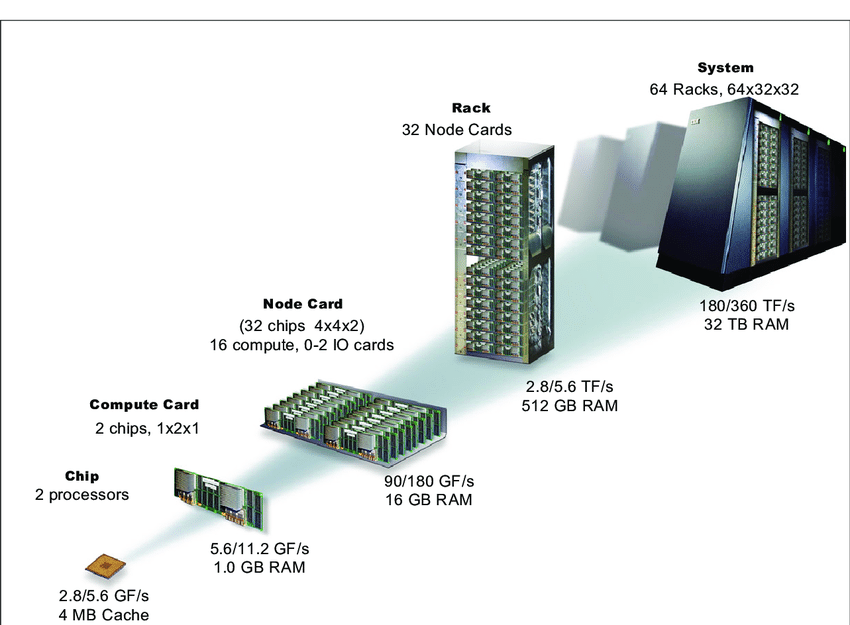
\includegraphics[width=0.8\textwidth]{img/ch6/BG_L_architecture.png}
    \caption{Architettura del super-calcolatore BlueGene/L}
    \label{fig:bgl_arch}
\end{figure}

Il file di log in ingresso BGLErrorLog.txt contiene $125624$ entry già filtrate, sono infatti riportate le entry relative ai soli errori fatali. Ogni entry ha il formato \textit{timestamp - nodo di origine - card di origine - messaggio di errore}.



\subsection{Temporal Coalescence}
Similmente a quanto fatto per Mercury, al fine di semplificare l'analisi dei log del sistema è stata applicata la tecnica della coalescenza temporale raggruppando le entry riconducibili allo stesso fault secondo una determinata finestra temporale $W$, determinata, anche in questo caso, tramite una \textit{Sensitivity Analysis}, calcolando il numero di tuple generate a seconda di multipli valori della \textit{window size}.

\begin{figure}[H]
    \centering
    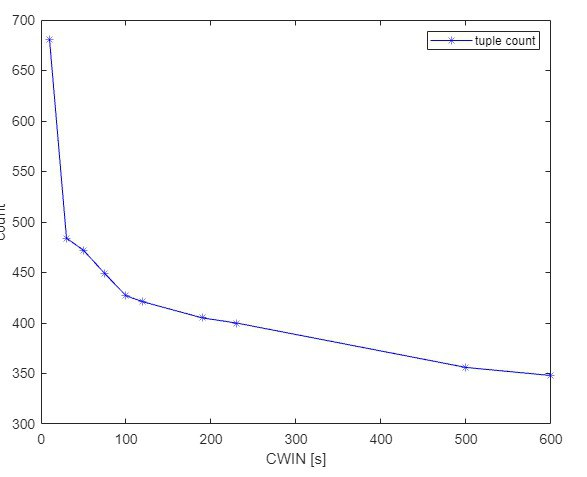
\includegraphics[width=0.8\textwidth]{img/ch6/blg_cwin.png}
    \caption{}
    \label{fig:blg_cwin}
\end{figure}

Ponendoci leggermente a destra del punto di knee sono stati scelti i seguenti valori per $W$:
\begin{itemize}
    \item $W=180$
    \item $W=220$
\end{itemize}

Per entrambe le \textit{window size} sono state generate le tuple e le seguenti statistiche:
\begin{itemize}
    \item Interarrivals: tempi di interarrivo tra le tuple (TTF).
    \item Starting points: timestamp del punto di inizio della tupla.
    \item Lengths: durata dei fallimenti e quindi la lunghezza delle singole tuple.
\end{itemize}


\subsection{Reliability}
Procediamo dunque con una stima empirica della reliability del sistema utilizzando il TTF calcolato a partire dagli \textit{interarrivals} ottenuti tramite l'analisi riportata nella sezione precedente.
In \cref{fig:bgl_reliability} è possibile notare come la reliability con $W=180$ sia migliore di quella con $W=220$. 
\begin{figure}[H]
    \centering
    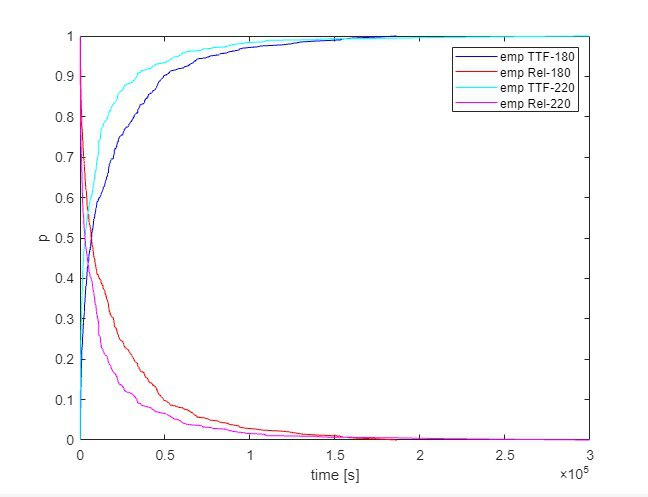
\includegraphics[width=\textwidth]{img/ch6/blg_ttf.png}
    \caption{Reliability BlueGeen/L con $W=180$ e $W=220$}
    \label{fig:bgl_reliability}
\end{figure}

Considerando la TTF e la Reliability empirica per $W=180$, è stata effettuata un'analisi per trovare la distribuzione che meglio rappresenta la Reliability empirica del super-calcolatore BlueGeen/L, con lo scopo di comprendere la natura dei fallimenti presenti nel sistema.

Anche in questo caso è stato provato il \textit{fitting} per le seguenti distribuzioni:
\begin{itemize}
    \item \textbf{Esponenziale} (\cref{fig:blg_fit_exp}): i fallimenti sono \textit{memory less} e con \textit{failure rate} costante;
    \item \textbf{Iper-esponenziale }(\cref{fig:blg_fit_iperexp}): i fallimenti sono dovuti a più cause tra loro indipendenti;
    \item \textbf{Weibull}(\cref{fig:blg_fit_weibull}): con questa
    distribuzione si modellano i fallimenti con memoria di componenti
    elettronici;
\end{itemize}

\begin{figure}[H]
    \centering
    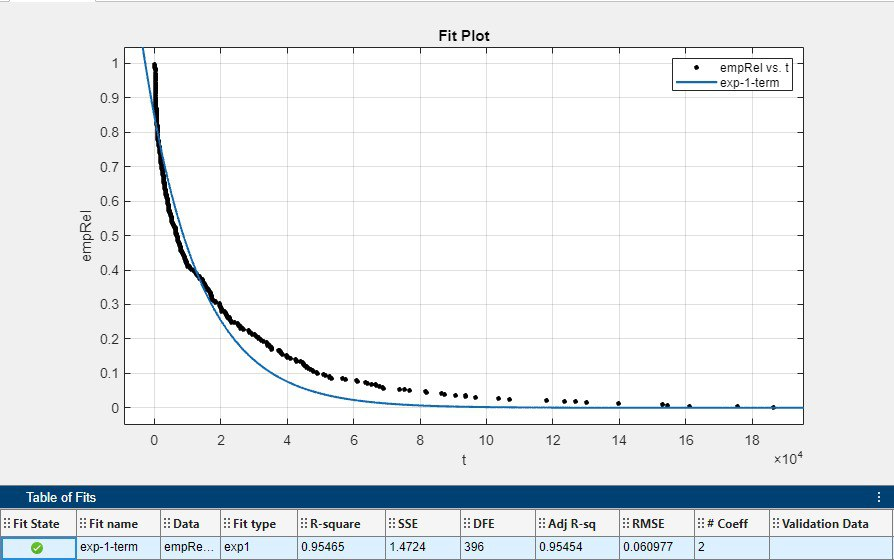
\includegraphics[width=\textwidth]{img/ch6/blg_fit_exp.png}
    \caption{Fit realiability BlueGeen/L con una distribuzione esponenziale}
    \label{fig:blg_fit_exp}
\end{figure}

\begin{figure}[H]
    \centering
    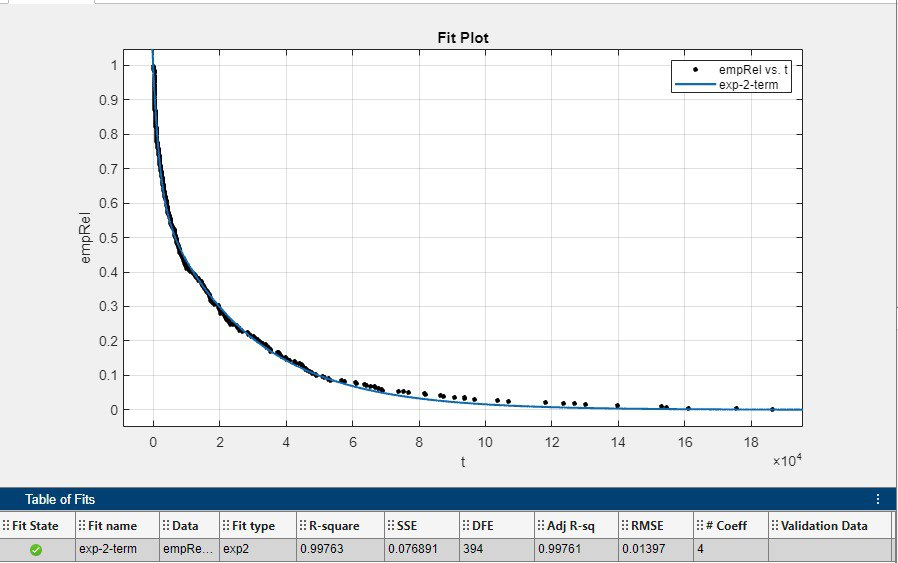
\includegraphics[width=\textwidth]{img/ch6/blg_fit_iperexp.png}
    \caption{Fit realiability BlueGeen/L con una distribuzione iper-esponenziale}
    \label{fig:blg_fit_iperexp}
\end{figure}

\begin{figure}[H]
    \centering
    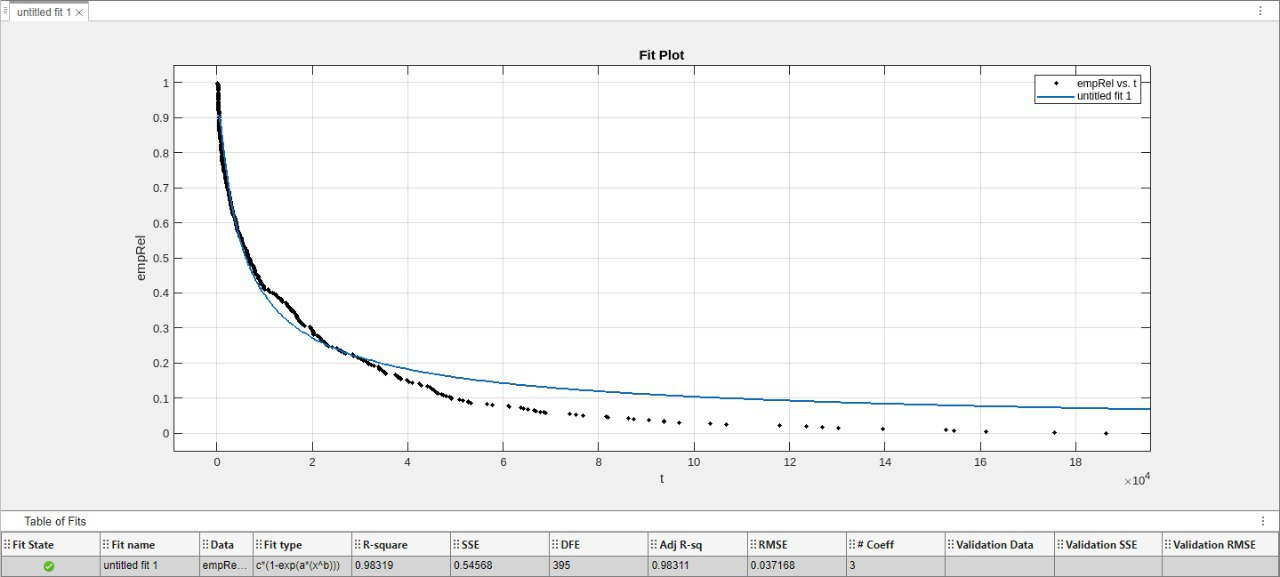
\includegraphics[width=\textwidth]{img/ch6/blg_fit_weibull.png}
    \caption{Fit realiability BlueGeen/L  con una distribuzione Weibull}
    \label{fig:blg_fit_weibull}
\end{figure}

\begin{table}[H]
\centering
    \begin{tabular}{|c|c|c|}
    \hline
    \multicolumn{1}{|c|}{\textbf{Curva}} &
    \multicolumn{1}{|c|}{\textbf{$R^2$}} &
    \multicolumn{1}{|c|}{\textbf{SSE}}
    \tabularnewline \hline

Esponenziale & $0.9546$ & $1.4724$   \tabularnewline \hline
Iper-esponenziale & $0.9976$ &  $0.0768$  \tabularnewline\hline
Weibull & $0.9832$ &  $0.5457$  \tabularnewline\hline

\end{tabular}
\caption{$R^2$ e SSE ottenuti dal fitting delle distribuzioni esponenziali ed iper-esponenziali}
\label{tab:blg_fit_parameters}
\end{table}


Osservando i valori relativi l'\textit{R-Square} e la SSE in \cref{tab:blg_fit_parameters},  è possibile affermare che la distribuzione che meglio approssima la reliability empirica è una iper-esponenziale. 

Come ulteriore conferma è stato effettuato il test di Kolmogorov-Smirnov per le due distribuzioni.

\begin{table}[H]
\centering
    \begin{tabular}{|c|c|c|}
    \hline
    \multicolumn{1}{|c|}{\textbf{Curva}} &
    \multicolumn{1}{|c|}{\textbf{H}} &
    \multicolumn{1}{|c|}{\textbf{P-Value}}
    \tabularnewline \hline

Esponenziale & $1$ & $2.7130 \cdot10^{-4}$   \tabularnewline \hline
Iper-esponenziale & $0$ &  $0.8016$  \tabularnewline \hline
Weibull & $0$ &  $0.10$  \tabularnewline \hline
\end{tabular}
\caption{Esito test Kolmogorov-Smirnov}
\label{tab:ks_blg}
\end{table}

\subsection{Analisi Collisions \& Truncations}

Proseguendo con $W=180$, sono state effettuate analisi per trovare collisioni e troncamenti all'interno delle tuple.

Per trovare una probabile collisione sono state esaminate le tuple a lunghezza maggiore, cercando eventi apparentemente slegati tra loro. 

Una probabile collisione è mostrata in \cref{fig:blg_collision} nella tupla 145, dove è possibile notare che le entry riportate in essa, stampate da card di I-O, non solo facciano riferimento a nodi appartenenti a Rack diversi (\textit{R62 ed R63}) ma sembrerebbero tra loro non correlate, in particolare i primi riportano un errore riconducibile ad un percorso errato o ad un file mancante, i restanti invece riportano un errore relativo alla dimensione eccessiva di un file.
\begin{figure}[H]
    \centering
    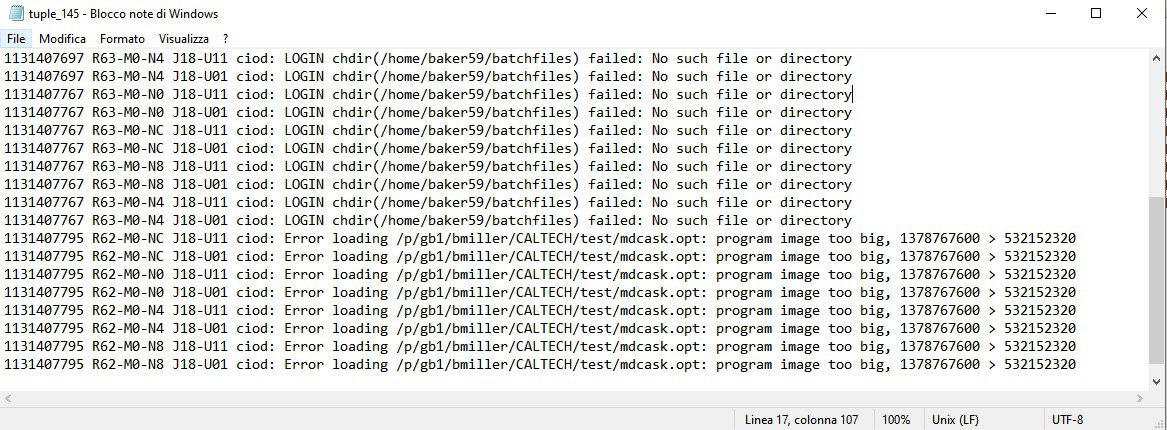
\includegraphics[width=\textwidth]{img/ch6/blg_collision.png}
    \caption{Esempio di probabile collisione per BlueGeen/L con $W=180$}
    \label{fig:blg_collision}
\end{figure}

Un esempio di probabile \textit{truncation} è mostrato in \cref{fig:blg_truncation} in cui è riportato il contenuto delle tuple $369,370,371,372$. Le entry riportate in esse riportano lo stesso messaggio d'errore e sono stampate dagli stessi nodi in un intervallo di tempo relativamente piccolo. 
\begin{figure}[H]
    \centering
    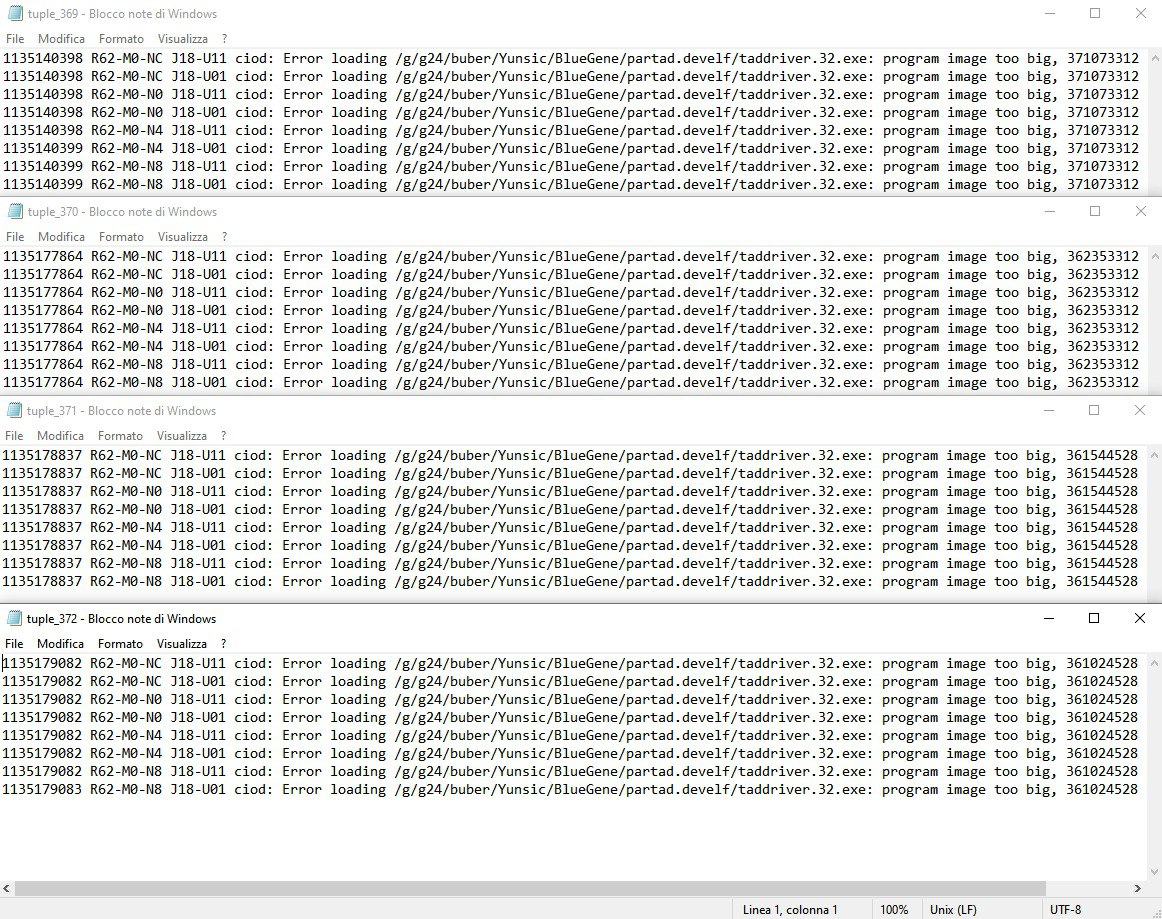
\includegraphics[width=0.8\textwidth]{img/ch6/blg_truncation.png}
    \caption{Esempio di probabile troncamento per BlueGeen/L con $W=180$}
    \label{fig:blg_truncation}
\end{figure}

\subsection{Ulteriori Analisi}
\paragraph{Studio della Window size per nodi}
Si vuole stabilire se sia possibile usare la stessa $W$ per i diversi nodi di BlueGeen/L. 

Dopo una fase di filtraggio sono stati identificati i quattro nodi con più errori del sistema, ed è stata svolta una sensitivity analysis simile a quella presente nelle sezioni precedenti. 
I nodi scelti sono:
\begin{itemize}
    \item R71-M0-N4
    \item R12-M0-N0 
    \item R63-M0-N2
    \item R03-M1-NF
\end{itemize}

Dai risultati in \cref{fig:comp_windows-size_per-nodo_bgl} è possibile notare come il valore $W=230$ potrebbe essere una scelta ottimale per la \textit{window size} per i nodi $R71-M0-N4,R12-M0-N0,R03-M1-NF$. Tuttavia osservando il grafico relativo al nodo $R63-M0-N2$ intuiamo come tale scelta potrebbe aumentare i fenomeni di collision delle entry non correlate nelle tuple rispetto ad una \textit{window size} più piccola per gli errori stampati. Ciò varrebbe per le sole entry stampate da questo specifico nodo.

\begin{figure}[H]
    \centering
    \begin{subfigure}{.5\textwidth}
        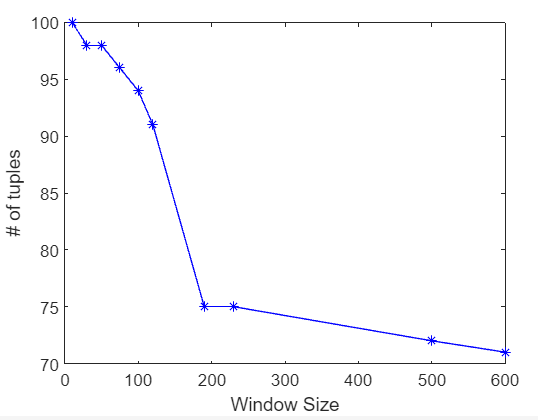
\includegraphics[width=\linewidth]{img/ch6/R71-M0-N4_cwin_numTuple.png}
        \caption{Nodo R71-M0-N4}
    \end{subfigure}\hfil
    \begin{subfigure}{.5\textwidth}
         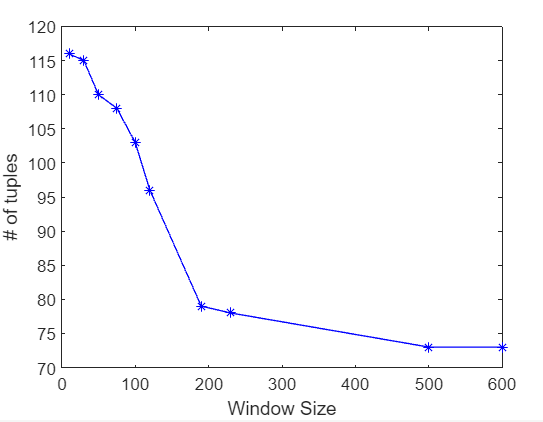
\includegraphics[width=\textwidth]{img/ch6/R12-M0-N0_cwin_numTuple.png}
         \caption{Nodo R12-M0-N0}
    \end{subfigure}

    \begin{subfigure}{.5\textwidth}
        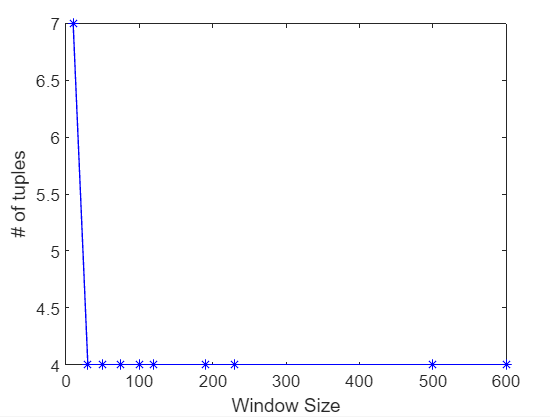
\includegraphics[width=\linewidth]{img/ch6/R63-M0-N2_cwin_numTuple.png}
        \caption{Nodo R63-M0-N2}
    \end{subfigure}\hfil
    \begin{subfigure}{.5\textwidth}
         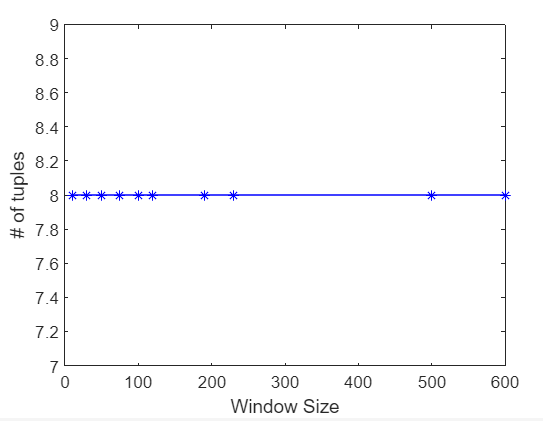
\includegraphics[width=\textwidth]{img/ch6/R03-M1-NF_cwin_numTuple.png}
         \caption{Nodo R03-M1-NF}
    \end{subfigure}
    \caption{Comparazione window size per nodo}
    \label{fig:comp_windows-size_per-nodo_bgl}
\end{figure}

\paragraph{Relazione tra system reliability e node reliability}
l fine di comparare la reliability del sistema a quella dei nodi è stata effettuata un'analisi del TTF-empirico per questi ultimi, a partire dagli interarrivals filtrati. 

Come nelle sezioni precedenti, è stata effettuata in seguito una procedura di fitting, al termine della quale sono state individuate $4$ curve iper-esponenziali, rappresentanti le reliability dei nodi.

In \cref{fig:bgl_comp}, è possibile notare come ci sia una sovrapposizione tra le reliability di BG/L con R12-M0-N0 ed R03-M1-NF con R71-M0-N40.
Gli altri nodi si trovano al di sopra della reliability del sistema.

\begin{figure}[H]
    \centering
    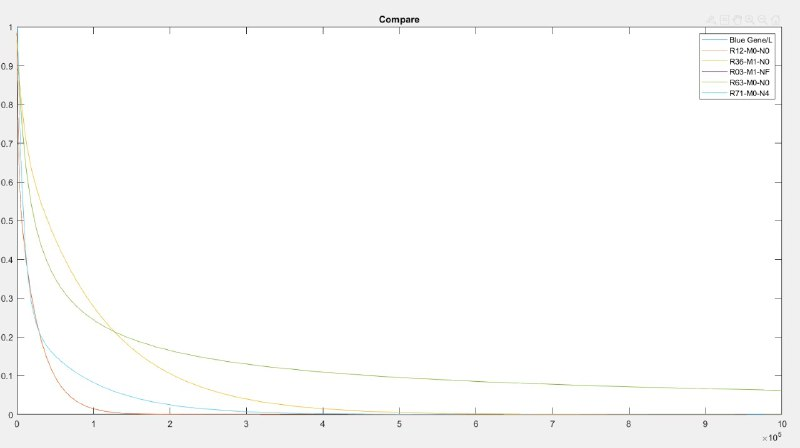
\includegraphics[width=.9\textwidth]{img/ch6/bgl_rel_comp.png}
    \caption{Confronto reliability nodi con quella del sistema per BlueGeen/L}
    \label{fig:bgl_comp}
\end{figure}


\paragraph{Dependability Bottleneck}

Dalle statistiche raccolte sui log di BGL i nodi più fallimentari risultano essere R71-M0-N4 e R12-M0-N0. 
È da notare che la gran parte dei fallimenti è da imputare alla scheda J18, responsabile delle operazioni di I/O, che può essere considerata il bottleneck del sistema. 

Per il resto i fallimenti sono distribuiti in maniera più bilanciata tra gli altri nodi rispetto a Mercury.





